\chapter{Lorem ipsum dolor sit amet}\label{cap:exampleChapter}
% ---
\section{Aliquam vestibulum fringilla lorem}
% ---

\lipsum[1]

% Exemplo de inclusão de figura
\begin{figure}[h]\label{fig:logo-ifce-sem-nome}
	\begin{center}
		
\includegraphics[width=4cm]{logo-ifce-sem-nome}
		\caption{Logomarca do IFCE sem nome}
	\end{center}
\end{figure}
% ------
\lipsum[2-3]

\includetable{tabela-exemplo} % Exemplo de inclusão de tabela

\lipsum[2-3]
% Exemplo de inclusão de gráficos
\begin{figure}
    \centering
    \begin{subfigure}[b]{0.45\textwidth}
        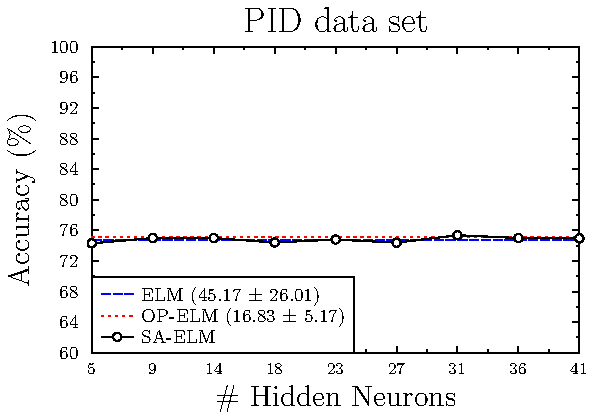
\includegraphics[width=\textwidth]{pid}
        \caption{Base de dados PID}
        \label{fig:pid}
    \end{subfigure}
    ~ 
    \begin{subfigure}[b]{0.45\textwidth}
        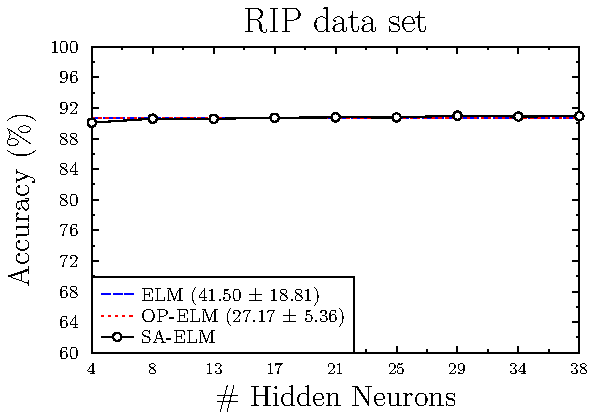
\includegraphics[width=\textwidth]{rip}
        \caption{Base de dados RIP}
        \label{fig:rip}
    \end{subfigure}
    \caption{Exemplo de gráfico}\label{fig:animals}
\end{figure}
% ------
\lipsum[2]

\begin{algorithm}
\caption{Algoritmo de exemplo}\label{bogosort}
  \begin{algorithmic}[1]
  \Procedure{Bogosort}{array}
    \While{\Not \Call{Está\_ordenado}{array}}
    \State array $\gets$ \Call{Permutação\_aleatória}{array} \Comment{Isso vai demorar muito :(}
    \EndWhile
  \EndProcedure
  \end{algorithmic}
\end{algorithm}

\lipsum[1]